% Sumber gambar figures/alur-penelitian.pdf (contoh \includegraphics).
% Kompilasi ulang hanya bila gambar diubah: xelatex alur-penelitian.tex
\documentclass[tikz,border=2pt,12pt]{standalone}
\begin{document}
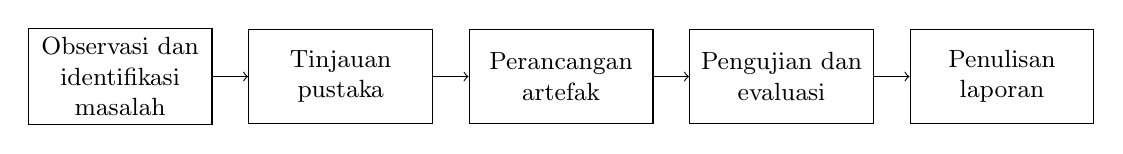
\begin{tikzpicture}[x=1cm,y=1cm,
    tahap/.style={draw,rectangle,align=center,text width=2.1cm,
      minimum height=1.2cm,font=\small}]
  \node[tahap] (a) at (0,0)  {Observasi dan\\identifikasi\\masalah};
  \node[tahap] (b) at (2.8,0) {Tinjauan\\pustaka};
  \node[tahap] (c) at (5.6,0) {Perancangan\\artefak};
  \node[tahap] (d) at (8.4,0) {Pengujian dan\\evaluasi};
  \node[tahap] (e) at (11.2,0) {Penulisan\\laporan};
  \foreach \p/\q in {a/b,b/c,c/d,d/e} \draw[->] (\p) -- (\q);
\end{tikzpicture}
\end{document}
